%%%%%%%%%%%%%%%%%%%%%%%%%%%%%%%%%
%
%       EXERCÍCIO
%
%%%%%%%%%%%%%%%%%%%%%%%%%%%%%%%%%

\ifdefstring{\atividade}{prova}{%
    \ifdefstring{\modo}{objetivo}{%
        \renewcommand{\valorquestao}{\ValorQObj\ ponto}
    }{%
        \renewcommand{\valorquestao}{\ValorQDisc\ pontos}
    }%
}%

\begin{exercicioBanco}[\valorquestao]
A curva abaixo representa o gráfico da função \(f(x) = \log_{2}(x)\), com \(x > 0\). Calcule a soma das áreas dos retângulos destacados.

\begin{center}
    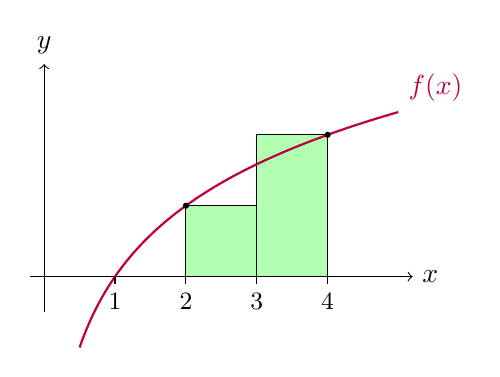
\begin{tikzpicture}[scale=0.9]
        % Eixos
        \draw[->] (-0.2,0) -- (5.2,0) node[right] {$x$};
        \draw[->] (0,-0.5) -- (0,3) node[above] {$y$};

        % Retângulos (usando a altura f(2), f(3), f(4))
        \fill[green!30] (2,0) rectangle (3,{ln(2)/ln(2)});
        \fill[green!30] (3,0) rectangle (4,{ln(4)/ln(2)});

        % Contornos dos retângulos
        \draw (2,0) rectangle (3,{ln(2)/ln(2)});
        \draw (3,0) rectangle (4,{ln(4)/ln(2)});
        
        % Função y = log2(x)
        \draw[domain=0.5:5, smooth, samples=200, thick, purple] plot (\x, {ln(\x)/ln(2)}) node[above right] {\(f(x)\)};

        % Pontos no gráfico
        \foreach \x in {2,4}
            \filldraw[black] (\x,{ln(\x)/ln(2)}) circle (1pt);

        % Marcas nos eixos
        \foreach \x in {1,2,3,4}
            \draw (\x,0) -- (\x,-0.1) node[below] {\small \x};
    \end{tikzpicture}
\end{center}
 
% Define as alternativas
\newcommand{\alternativas}{%
    \begin{center}
        \begin{tabularx}{\textwidth}{XXXXX}
            (a) \(2\). &
            (b) \(2,5\). &
            (c) \(3\). &
            (d) \(3,5\). &
            (e) \(4\).
        \end{tabularx}
    \end{center}
}

% Define a resposta correta
\newcommand{\resposta}{C}

% Lógica condicional para exibição
\ifdefstring{\atividade}{lista}{%
    \alternativas
    \vspace{0.5em}
    
    \noindent\textbf{Resposta:} letra \textbf{\resposta}.
}{%
    \ifdefstring{\modo}{objetivo}{%
        \alternativas
    }{%
        % modo = discursiva → não mostra alternativas
    }
}
\end{exercicioBanco}

